% Options for packages loaded elsewhere
\PassOptionsToPackage{unicode}{hyperref}
\PassOptionsToPackage{hyphens}{url}
%
\documentclass[
]{book}
\usepackage{lmodern}
\usepackage{amssymb,amsmath}
\usepackage{ifxetex,ifluatex}
\ifnum 0\ifxetex 1\fi\ifluatex 1\fi=0 % if pdftex
  \usepackage[T1]{fontenc}
  \usepackage[utf8]{inputenc}
  \usepackage{textcomp} % provide euro and other symbols
\else % if luatex or xetex
  \usepackage{unicode-math}
  \defaultfontfeatures{Scale=MatchLowercase}
  \defaultfontfeatures[\rmfamily]{Ligatures=TeX,Scale=1}
\fi
% Use upquote if available, for straight quotes in verbatim environments
\IfFileExists{upquote.sty}{\usepackage{upquote}}{}
\IfFileExists{microtype.sty}{% use microtype if available
  \usepackage[]{microtype}
  \UseMicrotypeSet[protrusion]{basicmath} % disable protrusion for tt fonts
}{}
\makeatletter
\@ifundefined{KOMAClassName}{% if non-KOMA class
  \IfFileExists{parskip.sty}{%
    \usepackage{parskip}
  }{% else
    \setlength{\parindent}{0pt}
    \setlength{\parskip}{6pt plus 2pt minus 1pt}}
}{% if KOMA class
  \KOMAoptions{parskip=half}}
\makeatother
\usepackage{xcolor}
\IfFileExists{xurl.sty}{\usepackage{xurl}}{} % add URL line breaks if available
\IfFileExists{bookmark.sty}{\usepackage{bookmark}}{\usepackage{hyperref}}
\hypersetup{
  pdftitle={A Minimal Book Example},
  pdfauthor={Yihui Xie},
  hidelinks,
  pdfcreator={LaTeX via pandoc}}
\urlstyle{same} % disable monospaced font for URLs
\usepackage{longtable,booktabs}
% Correct order of tables after \paragraph or \subparagraph
\usepackage{etoolbox}
\makeatletter
\patchcmd\longtable{\par}{\if@noskipsec\mbox{}\fi\par}{}{}
\makeatother
% Allow footnotes in longtable head/foot
\IfFileExists{footnotehyper.sty}{\usepackage{footnotehyper}}{\usepackage{footnote}}
\makesavenoteenv{longtable}
\usepackage{graphicx}
\makeatletter
\def\maxwidth{\ifdim\Gin@nat@width>\linewidth\linewidth\else\Gin@nat@width\fi}
\def\maxheight{\ifdim\Gin@nat@height>\textheight\textheight\else\Gin@nat@height\fi}
\makeatother
% Scale images if necessary, so that they will not overflow the page
% margins by default, and it is still possible to overwrite the defaults
% using explicit options in \includegraphics[width, height, ...]{}
\setkeys{Gin}{width=\maxwidth,height=\maxheight,keepaspectratio}
% Set default figure placement to htbp
\makeatletter
\def\fps@figure{htbp}
\makeatother
\setlength{\emergencystretch}{3em} % prevent overfull lines
\providecommand{\tightlist}{%
  \setlength{\itemsep}{0pt}\setlength{\parskip}{0pt}}
\setcounter{secnumdepth}{5}

\title{A Minimal Book Example}
\author{Yihui Xie}
\date{2020-02-18}

\begin{document}
\maketitle

{
\setcounter{tocdepth}{1}
\tableofcontents
}
\hypertarget{thesis-ferdinands}{%
\chapter{thesis Ferdinands}\label{thesis-ferdinands}}

Goal: evaluate performance of different models of the ASReview tool.

\hypertarget{stage-1-hyperparameter-optimization}{%
\subsection{Stage 1: hyperparameter optimization}\label{stage-1-hyperparameter-optimization}}

We are testing 5 models on 5 different datasets.

Every model has its own set of hyperparameters.
The hyperparameters are optimized on the 5 datasets in three different ways:

\begin{itemize}
\tightlist
\item
  1 on 1: maximum performance
\item
  4 on 1: cross-validation
\item
  5 on 1: more data = more better?
\end{itemize}

This results \((5+5+1)*5\) sets of hyperparameters.

\hypertarget{stage-2-simulation}{%
\subsection{Stage 2: simulation}\label{stage-2-simulation}}

for every for every model (5), for every dataset (5) and for every set of optimized hyperparameters (3), a simulation study is performed. From these \(5*5*3=75\) simulation studies, performance of the different models is evaluated.

\hypertarget{scripts}{%
\section{Scripts}\label{scripts}}

\begin{itemize}
\tightlist
\item
  simulatie:
\item[$\square$]
  script die optimalisatie genereert (config files.)
\item[$\square$]
  script die \texttt{.ini}'s voor simulatie genereert.
\end{itemize}

\hypertarget{strategy}{%
\chapter{Analysis strategy}\label{strategy}}

\hypertarget{datasets}{%
\section{Datasets}\label{datasets}}

\begin{itemize}
\tightlist
\item
  ptsd
\item
  ace
\item
  hall
\item
  nagtegaal - van PhD van Lars
\item
  medische van Jan
\end{itemize}

\hypertarget{models}{%
\section{Models}\label{models}}

(input table here?)

\begin{itemize}
\tightlist
\item
  Naive Bayes
\item
  Random Forests
\item
  Support Vecor Machine (doc2vec)
\item
  Logistic Regression
\item
  Dense Neural Network (doc2vec)
\end{itemize}

The other parameters remain fixed over the 5 models:

\begin{itemize}
\tightlist
\item
  Feature extraction = tf-idf
\item
  Query Strategy = max
\item
  Balance Strategy = triple
\item
  n\_instances=10 (number of papers each query)
\item
  n\_prior\_included = 5
\item
  n\_prior\_excluded = 5
\item
  mix\_ratio = 0.95 (95\% max, 5\% random)
\end{itemize}

\hypertarget{hyperparameters}{%
\section{Hyperparameters}\label{hyperparameters}}

\hypertarget{my-first-simulation}{%
\chapter{My first simulation}\label{my-first-simulation}}

\hypertarget{methods}{%
\section{Methods}\label{methods}}

A simulation study was performed on the Nagtegaal dataset, using a model with the following configurations:

\begin{itemize}
\tightlist
\item
  Model = Naive Bayes
\item
  Query Strategy = max\_random
\item
  Balance Strategy = Double
\item
  n\_instances=10 (number of papers each query)
\item
  n\_papers=2000 (shouldn't I do all?)
\item
  n\_prior\_included = 5
\item
  n\_prior\_excluded = 5
\item
  mix\_ratio = 0.95 (95\% max, 5\% random)
\end{itemize}

\begin{longtable}[]{@{}lllll@{}}
\toprule
Hyperparameters & & default & optimized &\tabularnewline
\midrule
\endhead
Model & & & &\tabularnewline
& alpha & 3.822 & 3.511844 &\tabularnewline
Balance & & & &\tabularnewline
& a & 2.155 & 0.254892 &\tabularnewline
& alpha & 0.94 & 1.459081 &\tabularnewline
& b & 0.789 & 0.394437 &\tabularnewline
Feature & & & &\tabularnewline
& ngram\_max & 1 & 2 &\tabularnewline
& split\_ta & 0 & 1 &\tabularnewline
\bottomrule
\end{longtable}

For the sake of evaluating the optimized hyperparameters, two simulations of five runs each were compared: one with default hyperparameters and with optimized hyperparameters.

\hypertarget{results}{%
\section{Results}\label{results}}

Explanation of the plots come from the \texttt{asreview-visualization} repository.
The optimized hyperparameters do not perform better than the default ones, this is probably due to the fact that the default hyperparameters have already been optimized in the past. It is therefore to know for which models this has already been done and which not!

\pagebreak

\hypertarget{inclusions}{%
\subsubsection{Inclusions}\label{inclusions}}

This figure shows the number/percentage of included papers found as a function of the
number/percentage of papers reviewed. Initial included/excluded papers are subtracted so that the line
always starts at (0,0).

The quicker the line goes to a 100\%, the better the performance.

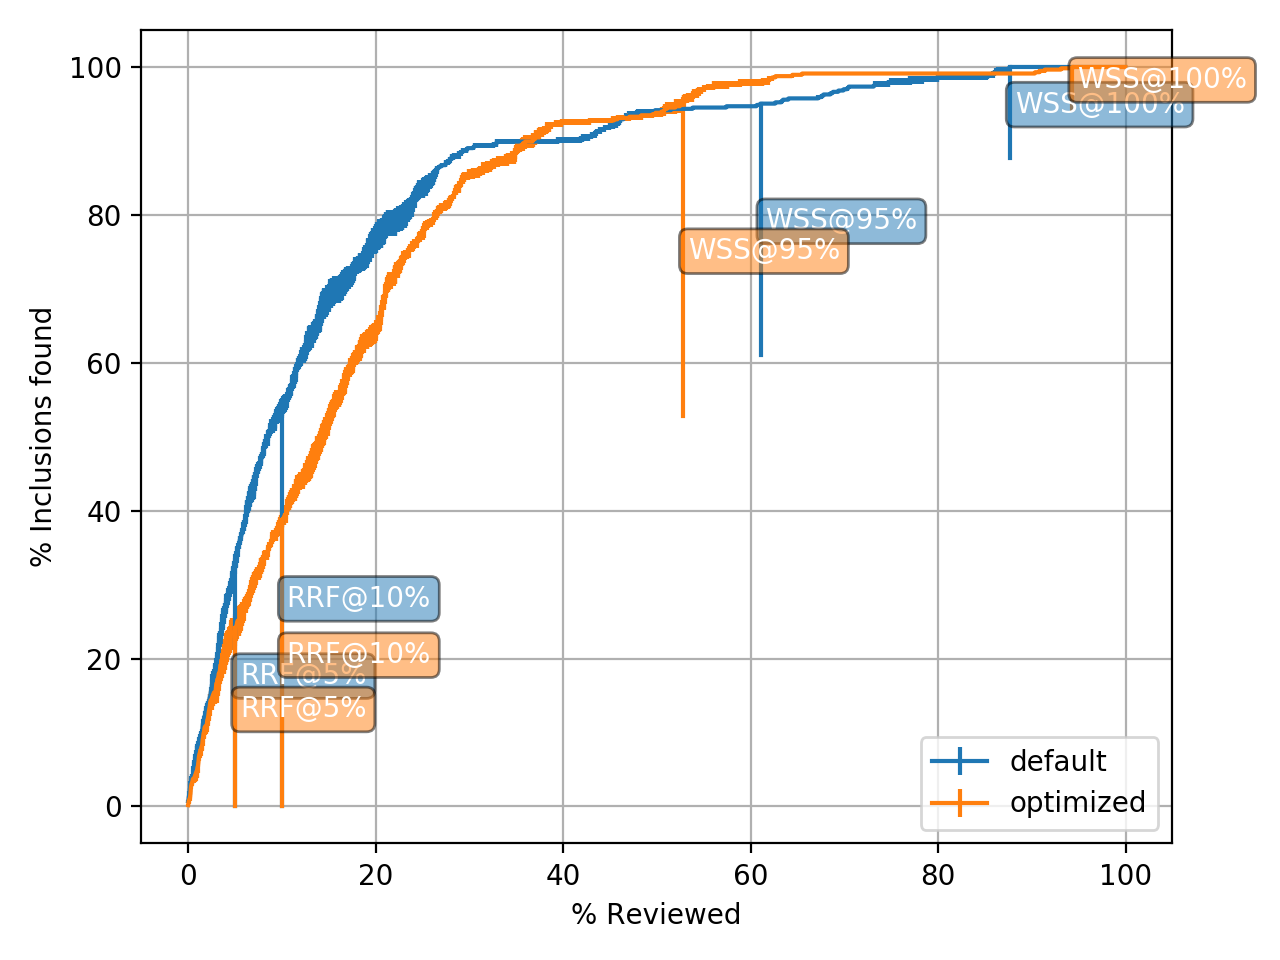
\includegraphics{figs/myfirstsim/Figure_1.png}

In the beginning, the model with default parameters finds inclusions quicker than the model with optimized hyperparamters.
Only after reviewing 50\% of the papers, the optimized hyperparameters outperform the default ones.

\pagebreak

\hypertarget{discovery}{%
\subsubsection{Discovery}\label{discovery}}

This figure shows the distribution of the number of papers that have to be read before discovering
each inclusion. Not every paper is equally hard to find.

The closer to the left, the better.

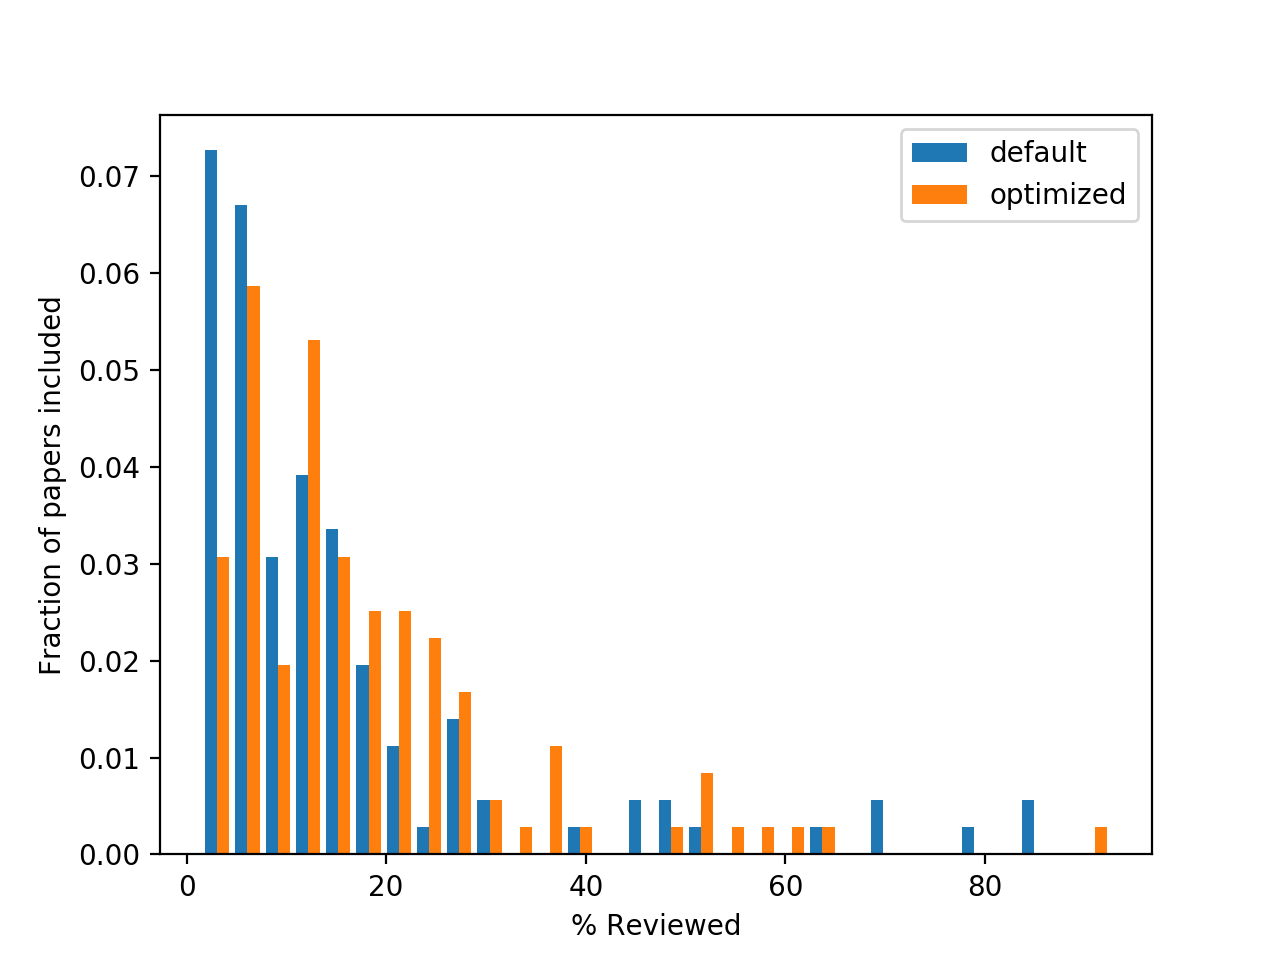
\includegraphics{figs/myfirstsim/Figure_2.png}

\pagebreak

\hypertarget{limits}{%
\subsubsection{Limits}\label{limits}}

This figure shows how many papers need to be read with a given criterion. A criterion is expressed
as ``after reading \emph{y} \% of the papers, at most an average of \emph{z} included papers have been not been
seen by the reviewer, if he is using max sampling.''. Here, \emph{y} is shown on the y-axis, while
three values of \emph{z} are plotted as three different lines with the same color. The three values for
\emph{z} are 0.1, 0.5 and 2.0.

The quicker the lines touch the black (\texttt{y=x}) line, the better.

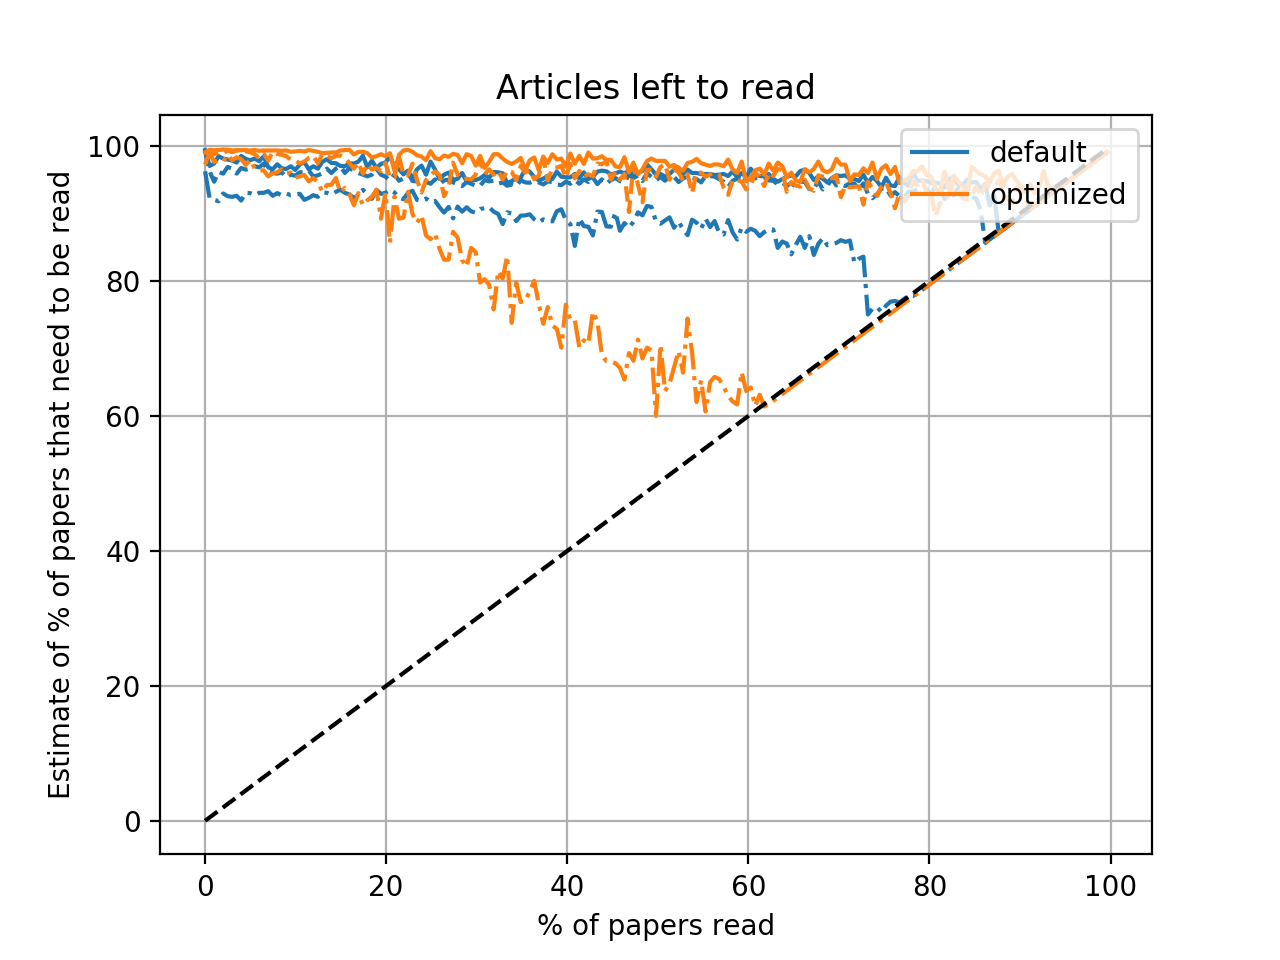
\includegraphics{figs/myfirstsim/Figure_3.png}

\pagebreak

\hypertarget{console-output}{%
\section{Console output}\label{console-output}}

3120 iterations ran overnight.

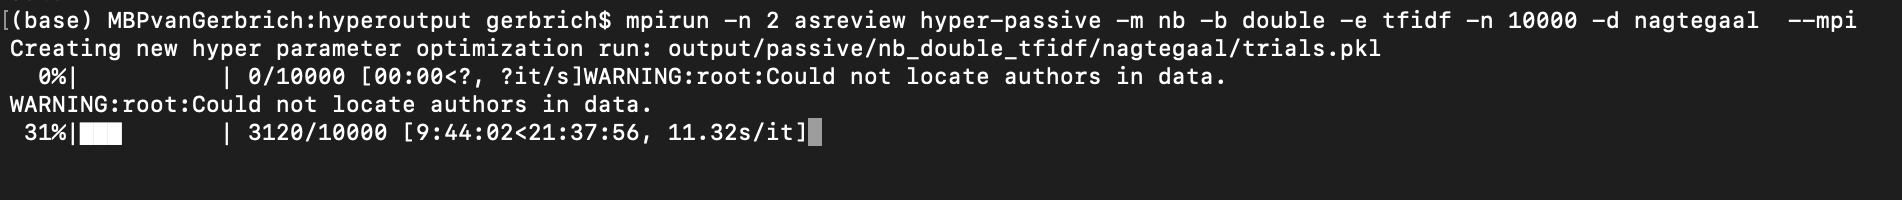
\includegraphics{figs/myfirstsim/computation.png}
2191 was best performing with a loss of 0.1124

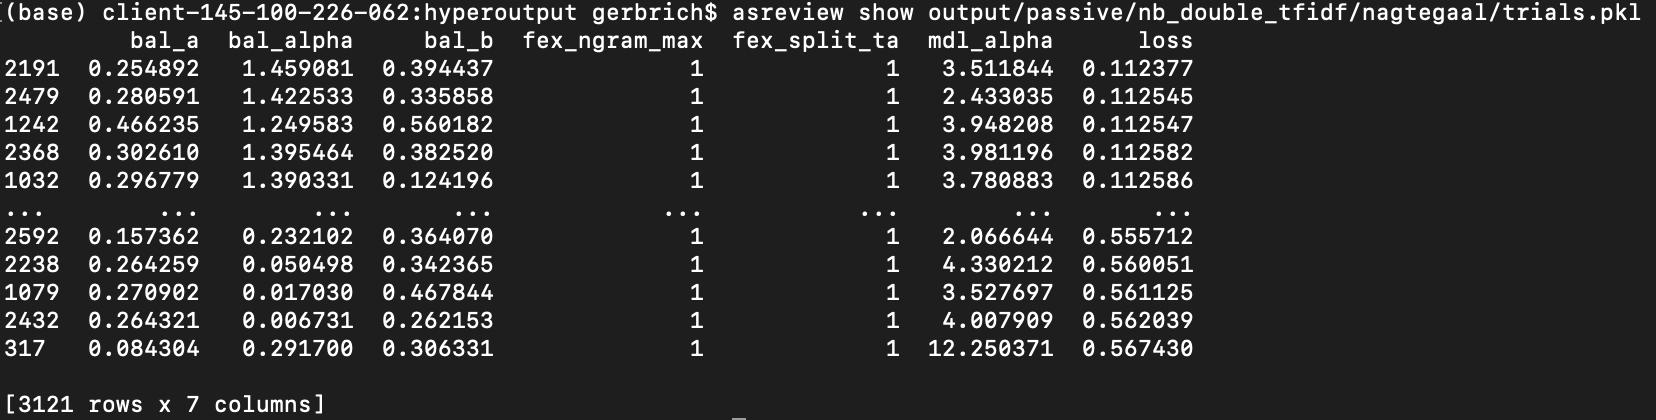
\includegraphics{figs/myfirstsim/optmizationresult.png}

\hypertarget{notes}{%
\section{Notes}\label{notes}}

\begin{itemize}
\item
  Optimizing the hyperparameters with the Nagtegaal set and then running a simulation on the Nagtegaal dataset is using the data twice.
  This leads to overfitting. A next approach could be to perform some way of cross-validation, e.g.~split the datasets in train and test datasets.
\item
  There are two main optimization modes: passive and active learning.
  The first is used here and is relatively fast, the second is more computationally expensive.
\item
  Of primary interest is the comparison of different model configurations in predictive performance.
  A simulation study can be performed with all possible configurations using the default hyperparameters.
  The results could be used to select model configurations that could possibly benefit from hyperparameter sreening.
\item
  Second, we could investigate how much is to gain in predictive performance from optimizing the hyperparameters.
  For this, some cross-validation strategy should be used.
  Optimization can consist of two steps:
  first, optimization through passive learning can be performed, from which the best performing models can be selected for the second step:
  optimization through passive learning.
\end{itemize}

\hypertarget{possible-research-questions}{%
\subsection{Possible Research Questions}\label{possible-research-questions}}

\begin{itemize}
\tightlist
\item
  Which model configurations have good predictive performance?

  \begin{itemize}
  \tightlist
  \item
    for what kind of data sets and under which circumstances?
  \end{itemize}
\item
  Does optimization of hyperparameters lead to substantial gain in predictive performance?

  \begin{itemize}
  \tightlist
  \item
    How much and why?
  \item
    How do the hyperparameters relate to one another?
  \item
    What is the optimal way to tune the hyperparameters?

    \begin{itemize}
    \tightlist
    \item
      to determine by cross-validation
    \item
      for example: optimize over a large number of datasets? or a different strategy?
    \end{itemize}
  \end{itemize}
\item
  \ldots{}
\item
  \ldots{}
\end{itemize}

\hypertarget{appendix-appendix}{%
\appendix}


\hypertarget{list-of-definitions}{%
\chapter{List of definitions}\label{list-of-definitions}}

\end{document}
